\section{Devices}
\label{sec:devices}

When describing his vision for Ubiquitous Computing, Weiser draws a parallel to the evolution of the electric engine:

\begin{quote}
    How do technologies disappear into the background? The vanishing of electric motors may serve as an instructive example.
    At the turn of the century, a typical workshop or factory contained a single engine that drove dozens or hundreds of
    different machines through a system of shafts and pulleys. Cheap, small, efficient electric motors made it possible first
    to give each tool its own source of motive force, then to put many motors into a single machine.\cite{weiser91}
\end{quote}

Electric engines are in some ways like computers, but in other ways entirely unlike them. Both have had a development where
they have shrunk dramatically in size, but unlike electric engines, computers perform more than one task. Comparing electric
engines to computers is like comparing processing units to machines -- one is nothing more than a component of something bigger.

A \emph{device} is an entity consisting of several components (processors, sensors, NFC chips, and more) that performs more
than one task. That is, unlike motion sensors, which only sense motion, a device is a collection of functionality in a single
computer. Devices are, in their very nature, anti-ubiquitous computers, as they demand attention, rather than become
invisible,\footnote{Weiser writes that ``multimedia tries to grab attention, the opposite of the ubiquitous computing ideal of
invisibility''\cite{weiser93}} and are in no way single-purpose.

Examples of devices are easy to find: laptops, personal computers, smartphones (in fact, mobile phones before the current generation
of smartphones were devices, too), and tablets. All of these perform the same, common
tasks (multimedia -- watching and reading; office work -- timekeeping, writing; etc.). They are the epitome of redundancy, and yet
they are very popular.\footnote{Cisco projects 3 devices per capita in the world by 2017.\cite{cisco}}

Whereas some modern tablets and TVs take similar forms to those of the early, ubiquitous pads and boards, they differ in being
centres attention, where pads and boards were designed to be invisible.

\subsection*{Co-existence}

Weiser does not claim that Ubiquitous Computing must be the only kind of computing present, for the ubiquitous state to be reached.
Rather, it will coexist with Personal Computing for a while, until it eventually becomes more popular and pushes Personal Computing
out of the picture (see Figure \ref{fig:trends-graph}).

\begin{figure}[htb]
	\centering
	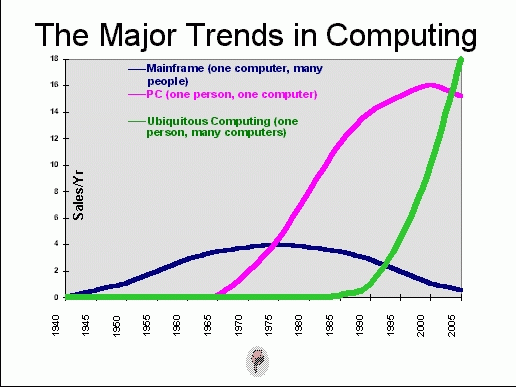
\includegraphics[width=0.75\textwidth]{multipurpose/trends-graph}
	\caption{Trends in computing, according to Weiser, depicting Ubiquitous Computing overtaking Personal Computing in sales around
		2004. This prediction was orignally made in 1996.\cite{weisernomadic}}
	\label{fig:trends-graph}
\end{figure}

Devices are a modern incarnation of Personal Computing, allowing personal computers to be accessed in more places. Devices are personal
computers inspired by the ever-presence of Ubiquitous Computing. The over-simplification used in Weiser's graph, indicating that only
Ubiquitous Computing can have several computers for one person, may cause confusion. Devices are in no way ubiquitous. Although they may
be many, they lack most of the other qualities present in ubiquitous computers. Each
of the most commonly used devices performs each of the most used tasks, providing both office tools and entertainment. As explained
previously, devices are not single-purpose, nor are they invisible.

We have, indeed, seen Ubiquitous Computing grow in popularity, with sensors, NFC chips, and the likes becoming increasingly used. But
at the same time we are seeing a competing trend take over some of the fields that were previously dominated by ubiquity: the trend of
devices.

Weiser predicted that the sales of personal computers would soon decline, but he had not anticipated the envigorating effect, the
coming of devices would have. In fact, the number of devices sold annually is far from declining (see Figure \ref{fig:actual-sales-graph}).

\begin{figure}[htb]
    \centering
    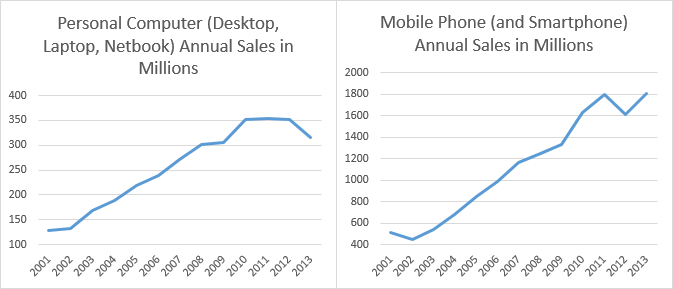
\includegraphics[width=1\textwidth]{multipurpose/actual-sales-graph}
    \caption{Annual Sales of two categories of devices (personal computers and mobile phones) on the increase for the last 10 years.
        Whereas the sale in personal computers has stagnated (and even declined) in recent years, this might to some extent be
        explained by the introduction of tablets. The overall sales of devices seems to still be on the increase. (Note
        that more than 5 times as many mobile phones as personal computers are sold.)\cite{wikipedia-mobiles}\cite{wikipedia-pcs}\protect\footnotemark}
    \label{fig:actual-sales-graph}
\end{figure}

\footnotetext{The graphs are based on an aggregation of data maintained on Wikipedia. While Wikipedia is not itself necessarily a
credible source, it does provide some sense of overview. The graphs should not be seen as meticulously precise, but rather as
indicative of a tendency.}

Wearable technology seems like a natural extension of Ubiquitous Computing, as wearable technology naturally blends with the body
the user, and become invisible. A tiny device measures your pulse when you go running, and another tracks your location when going for a
walk.\footnote{Sources for old devices that did this, and only this, missing.} But despite there still being launched truly ubiquitous,
single-purpose, invisible, wearable technology (such as FitBit, a wearable fitness tracker\footnote{``Fitbit makes it easy to track
activity, sync stats, see trends and reach goals.'' (http://www.fitbit.com.)}) there is a conflicting tendency towards gathering as much
functionality as possible in a few devices. An example of this tendency is Apple's upcoming iWatch, a device worn on your wrist, which
could indeed track things such as pulse and location.\footnote{Source on iWatch!} Such a device --- providing both communication,
various tracking, and some office features --- makes computers like the FitBit obsolete, just like GPS tracking in mobile phones to a
large extent forces single-purpose GPS trackers out of the market.

There are many more possibilities for devices to provide seemingly ubiquitous experiences that would not have been feasible as stand-alone
computers. For example, smartphones are starting to ship with NFC built-in\footnote{For example, Samsung Galaxy S5 has NFC (although it is
a feature well-hidden). (http://www.samsung.com/global/microsite/galaxys5/specs.html)}, which will allow them to take over much of the
functionality that was previously handled by access cards.

Credit cards have recently been the field of many new ideas, too, striving to make the interaction with them more ubiquitous. Visa has developed
a technology for contactless payment, allowing customers to pay without having to enter a PIN.\footnote{``Visa payWave lets you breeze through
check out faster since you don't need to fumble for cash. Simply wave your card in front of a secure reader and you’re on your way.''
(http://usa.visa.com/personal/security/card-technology/visa-paywave.jsp)} The idea of making payment easier is taken further by Coin, which
allows users to have a single card that can be used as any of the cards they own.\footnote{``It's a simple card, just like a regular payment
card. You can swipe it just like any other card. The difference between a Coin and any other card: all of these cards are inside my Coin.
(https://onlycoin.com/)} This removes another hindrance for users prone to fumbling with cards in their wallets. Coin uses a smartphone as card
manager, making it a piece of Ubiquitous Computing that is heavily device dependent. It is not a far stretch to imagine smartphones in the
future taking it a step further and simply integrate the required chips to make them work as credit cards.

In fact some steps have been taken towards making payment from smartphones simple. Danske Bank's MobilePay makes it possible to transfer money
to a recipient by knowing only their phone number. This is hardly a ubiquitous experience, as it requires bringing out a device and giving it
some real attention. The focus of the transaction is on the tool, getting the recipients phone number, and entering the correct payment
amount.\footnote{(http://www.danskebank.dk/mobilepay)}

The tendency seems to be that \emph{new things to measure} and \emph{new ways to measure} start out as truly ubiquitous computers, that do
nothing more than measure and communicate, until the idea becomes popular enough to be scooped up in a very un-ubiquitous device. I will
not make Weiser's mistake of trying to predict what will happen in the future, but for now Ubiquitous Computing remains but a tiny speck in the
grand scheme of computing.

It is not the case that all Ubiquitous Computing is disappearing, but rather
that ubiquity is only desirable for a few, specific areas. Sensors that track movement (for example to turn on patio lights) are not going to be integrated
into devices, and it is indeed an advantage that these sensors are out of sight.

For the vast majority of features, however, devices dominate, and Weiser's quote from 1991 is as true today as it was in its
time: ``Today's multimedia machine makes the computer screen into a demanding focus of attention rather than allowing it to fade into the
background.''\cite{weiser91} I would argue that this happens because the end-user wants to be in control of the technology, and that
computers that demand attention are indeed desirable.

\subsection*{Choice}

The uprising of devices results in the ever-presence of computers being less of the \emph{inescapable} kind and more of the \emph{accessible}
kind. Paraphrasing the words of a popular fast-food chain, ``Choice is King''\footnote{Burger King used the phrase ``Taste is King'' as a campaign slogan. (http://www.bk.com/)}.

Users want to be able to take things with us. Users want to be able to put things down and leave them behind. This is what makes Ubiquitous Computing undesirable.
What is by Weiser described as a great future, full of possibilities, would be dreaded by many:

\begin{quote}
    Doors open only to the right badge wearer, rooms greet people by name, telephone calls can be automatically forwarded to
    wherever the recipient may be, receptionists actually know where people are, computer terminals retrieve the preferences
    of whoever is sitting at them and appointment diaries write themselves.\cite{weiser91}
\end{quote}

Feeling constantly watched, with no way of escaping the surveillance, is by no means something most people dream about.
Functionality condensed in devices is such a popular meme exactly because people want a way to leave the computers behind.
People crave the possibility of choice. They will most likely not choose the leave the computer behind, but they want to
be able to.

Google makes its business primarily thorugh facilitating advertising for other companies. They gather information on users of
their search engine and other services (including email, social network, and calendar). This information is used to target ads
at their users in such a way that the users get the ads they are most likely to interact with.

The services Google provide are very like those described by Weiser above. The relationship between Google and their customers
is like that between devices and their users. Not all users are the same: some share everything; some have a policy regarding
what they share; and some share nothing at all. What they all have in common is the ability to put down the device, delete their
Google account, and leave the computers behind.\footnote{I think the reason for the popularity of services provided by companies
that provide a full package (Microsoft, Apple, Google) can be explained by much the same kind of thinking that makes devices so
popular.}

\textbf{Feeling secure during payments -- when it has to do with money...}